% sec_d2.tex -- d = 2 results of the HT_Pert note (from HT2dPert, 2026-10-14).
% Every number here has a replay row in repro_d2.tex / results_map.md (check ids p2.*); macros in numbers_d2.tex.
% Needs: amsmath, booktabs, graphicx. Inputs: fig_c4_delta_d2.pdf (make_fig_d2.py).
\section{Results in two dimensions}\label{d2:sec}

In $d=2$ the truncation is a level cutoff $\ell\le L$ and the coefficients are computed in three ways: a production solver
to eighth order for $L\le\HTpTwoLprod$, exact-rational and Cauchy-integral solvers at small $L$, and sums over intermediate
states that give $C_4(L)$ to $L=\HTpTwoLfour$ and $C_5(L)$ to $L=\HTpTwoLfive$. Through $\eps^3$ the truncation converges to the
continuum. At $\eps^4$ every window in use diverges like $\ln L$; a complete window, derived from the level budget of
divergent sub-bubbles, removes the logarithm and gives $C_4$ to $\HTpCfourTwoDev$. At $\eps^5$ it needs two further pieces
and then gives $C_5$ to $\HTpCfiveTwoDev$, if the data carry no residual $\ln L$ term (Sec.~\ref{d2:c5log}). $C_6$ to $C_8$ are not reproduced. Table~\ref{d2:tab:summary} collects the results, and Appendices~\ref{d2:app:eps4} to~\ref{d2:app:legs} give the derivations and the supporting data.

\begin{table}[ht]
\centering\small
\begin{tabular}{@{}llllp{3.1cm}@{}}
\toprule
 & HT, $L\to\infty$ & continuum & $|C_n^{\rm HT}/C_n-1|$ & status \\\midrule
$C_2$ & $\HTpCtwoTwo$ & $\frac49\log2$ & \HTpCtwoTwoDigits{} digits & final \\
$C_3$ & $\HTpCthreeTwo$ & $-0.8748500127$ & $\HTpCthreeTwoDev$ & final \\
$C_4$, complete window $W$ & $\HTpCfourTwo$ & $5.0488684314$ & $\HTpCfourTwoDev$ & final \\
$C_5$, scheme $W_{cs}$ (Sec.~\ref{d2:c5}) & $\HTpCfiveTwo$ & $-38.8336459$ & $\HTpCfiveTwoDev$ & final; no residual $\ln L$ assumed \\
$C_6$ to $C_8$ & not reproduced & $\NTwoCsixCont$, \dots & & not reproduced \\
\bottomrule
\end{tabular}
\caption{$d=2$ perturbative results. ``Final'' refers to the quoted value in the sense of Sec.~\ref{sec:refvals}: the
analysis is complete, with post hoc choices. The windows behind $C_4$ and $C_5$ were derived after their effects had been
seen, and the rules $W_c$ and $W_{cs}$ behind $C_5$ are provisional (Table~\ref{d2:tab:status}). Uncertainties are spreads
over tail models and fit windows, not standard errors; that of $C_4$ is the half spread of nine fits, rounded up
(Sec.~\ref{d2:c4}).
The $C_5$ uncertainty assumes that the data carry no residual $\ln L$ term. They cannot exclude one: with the bound
judged from the median of the fits it would move $C_5$ by up to about $\HTpCfiveTwoLog$, and the spread of single fits
would allow $-0.7$ to $+0.5$ (Sec.~\ref{d2:c5log}). Continuum values from Table~\ref{tab:refvals}; in $d=2$,
$C_3=\frac4{27}\log^22-\frac{\Gamma(1/4)^8}{324\pi^4}$ and $C_4=\frac1{648}\big[16P_4(2)-64\log^32-32\log2\,Q_2-359\zeta(3)\big]$,
with $Q_2=\frac{\Gamma(1/4)^8}{24\pi^4}=12.77138119864696$ and the primitive four-loop wheel value $P_4(2)=250.48731558186729$
(GFF note, section ``Finite multivariable representations for the nonprimitive masters'').}
\label{d2:tab:summary}
\end{table}

\subsection{Model and level cutoff}\label{d2:model}
On the unit circle the field has one oscillator $A_{ab}$ for each $a,b\ge0$, describing $\partial^a\bar\partial^b\phi$, with
energy $\Ds+a+b$, spin $a-b$ and weight
\begin{equation}
 \phi(\theta)=\sum_{a,b}\sqrt{w_{ab}}\,\big(e^{\mathrm i(a-b)\theta}A^\dagger_{ab}+e^{-\mathrm i(a-b)\theta}A_{ab}\big),\qquad
 w_{ab}=\frac{(\Ds)_a(\Ds)_b}{a!\,b!},\qquad \Ds=\tfrac12-\tfrac\eps4 .
 \label{d2:eq:modes}
\end{equation}
A Fock state has level $\ell=\sum(a+b)\,n_{ab}$ and particle number $P=\sum n_{ab}$, and its free energy is
$\ell+P\Ds=H_0+\eps F_1$, with $H_0=\ell+\frac P2$ and $F_1=-\frac P4$ (the $d=1$ Hamiltonian, Eq.~\eqref{eq:H}, has $H_0=\ell+\frac P4$). With
$M=\langle{:}\phi^2{:}\rangle_\theta$ and $V=\frac1{12}\langle{:}\phi^4{:}\rangle_\theta$,
\begin{equation}
 H(\eps)=H_0+\eps F_1+r(\eps)M+g(\eps)V+D ,
 \label{d2:eq:H}
\end{equation}
where $D$ is the window. We keep the states with $\ell\le L$ (even), spin zero and even under $a\leftrightarrow b$; the zero mode
$(0,0)$ costs no level and is not truncated; the other modes form the bath. $r$ and $g$ are tuned at cutoff $L$, and $C_n(L)$ follows from the reference
states $|p\rangle$, $p=0,\dots,3$, as in Sec.~\ref{sec:method}, with $C_0=1$, $C_1=-\frac16$, $r_1=0$, $g_1=\frac13$ at every $L$.
Through $\eps^8$ no intermediate state has more than $p+16$ particles, so this cap is exact. We write $Z=A_{00}+A_{00}^\dagger$,
$\chi=\phi-Z$ for the non-zero modes, $M'=M-{:}Z^2{:}$, and $\chi_{aa}$ for the one-quantum state of mode $(a,a)$.

\emph{Windows.} The raw truncation has $D=0$. The consistent window is the vacuum window
$D_L(\ell)=E_v(L)-E_v(L-\ell)$ with self-consistent vacua $E_v(\lambda)$ at sub-cutoffs $\lambda\le L$, each computed
with the same window. The literal window is the same difference with the vacua $E_v(\lambda)$ of the raw truncation; it
differs from the consistent window from $\eps^6$ on. The zero-mode window replaces $E_v$ by the self-consistent energy
$E_z(\lambda)$ of the channel with the same number $z$ of zero-mode quanta. All of them are diagonal.

\emph{Terms.} The zero-mode channel $|z\rangle=(A_{00}^\dagger)^z|0\rangle/\sqrt{z!}$ has free energy $E^0_z=\frac z2$;
$|z,\chi\rangle$ is a state with $z$ zero-mode quanta and bath part $\chi$ of level $\ell_\chi$, and $|k\rangle$ is an
intermediate state of free energy $E^0_k$. In a time-ordered product of vertices, a \emph{slice} is the intermediate state
between two neighboring vertices. A sub-process (a bubble, sunset or mass insertion) absorbs or emits some $\chi$ quanta,
its \emph{legs}; the other quanta present are \emph{spectators}, \emph{hard} if their level is comparable with $L$ and
\emph{soft} otherwise. A term of $M'$ with one creator and one annihilator is a \emph{hop}; one with two creators or two
annihilators is a \emph{pair} term. The \emph{exchange sunset} of $\chi_{aa}$ is the $\eps^2$ ordering in which the new
$\chi_{aa}$ is emitted, together with a bubble, before the old one is absorbed, so that two $(a,a)$ quanta are present at
once. An \emph{auxiliary channel} is the eigenvalue branch $E_z(\lambda)$, with right eigenvector $\psi_z(\lambda)$, of the
Hamiltonian at a sub-cutoff $\lambda\le L$ through $|z\rangle$; the windows use it as the reference for zero-mode clusters
inside larger states. A \emph{ket-referenced (Bloch)} effective interaction uses the energy denominators of the state it acts
on, so it is not symmetric in $z$ and $z'$. Newton's forward-difference form in $p$, $E_p=E_0+p\,e_1+\binom p2e_2+\dots$,
defines the \emph{Newton coefficients} $e_1=E_1-E_0$ and $e_2=E_2-2E_1+E_0$. A \emph{tower} is a fit model: a constant plus
terms $\ln^jL/L^k$ (Appendix~\ref{d2:app:c4exact}). A \emph{tagged} line is an external quantum replaced by a copy that the
cutoff and the windows see with an assigned level, its \emph{charge} (Appendix~\ref{d2:app:tag}).

\subsection{Solvers}\label{d2:solvers}
The production solver \code{code/lri\_d2\_coeff\_hpc/} computes $C_0$ to $C_8$, $r_n$, $g_n$ and every reference energy for
$L\le\HTpTwoLprod$ in the raw and consistent schemes, in float64 truncated power series in $\eps$ ($L=16$ to 30 on the symmetry cluster, 32 and 34
on SDSC Expanse); the literal window is implemented and checked at small $L$. Two clean-room solvers, written from the model specification without seeing the production code or each other,
check it: exact Rayleigh--Schr\"odinger perturbation theory in rational arithmetic ($L\le\NTwoRSLmax$) and Cauchy integrals of
the non-perturbative truncated Hamiltonian at complex $\eps$ with 256-bit arithmetic ($L\le\NTwoCauchyLmax$). The production
solver agrees with the exact one to $\HTpTwoImplAgree$ (largest scaled difference over all $C_n$, $r_n$, $g_n$, energies and
vacua, $n\le8$), and the Cauchy solver with the exact one to $\NTwoCauchyAgree$ (Sec.~\ref{d2:checks}).

The large-$L$ results come from separate codes in \code{code/lri\_2d\_coeff\_independent\_check/}. With $V$ and $M$ factorized
into zero-mode and $\chi$ parts, a $K$-vertex chain is a sum over $\chi$-line patterns of a Wick count, an exact zero-mode
path sum and a $\chi$ level sum; at $\eps=0$ the weights factorize holomorphically, $\sum_{ab}w_{ab}y^a\bar y^b=(1-y)^{-1/2}(1-\bar
y)^{-1/2}$, and the cutoff only bounds the largest slice level, so one run gives every even $L$. These codes reproduce the exact
rationals and the production solver: $C_2(L)$ and $C_3(L)$ to $\NTwoLowAgree$ (absolute), $C_4(L)$ to $\NTwoCfourAgree$ and
$C_5(L)$ to $\NTwoCfiveAgree$ (relative). The $C_5$ engine was later optimized; per task it agrees with the original to $\NTwoOptRegress$,
and the assembled $C_5(L)$ reproduces the earlier data at $L\le200$ to $\NTwoOptAssembly$.

The zero-mode scheme has its own exact solver (\code{zeromode\_exact/}, $L\le18$; Appendix~\ref{d2:app:c4exact}). Every
other window scheme at $L\le16$, and every descendant spacing, comes from two further exact solvers in the same package: \code{complete\_exact/} (scheme $W$ and its variants as explicit operators, exact through
$\eps^8$ for $L\le16$) and its copy \code{residual\_log/\allowbreak{}ce\_wc/} with rule $W_c$ and the external-line windows
(Appendix~\ref{d2:app:eps5data}).

\subsection{Second and third order}\label{d2:low}
At $\eps^2$ only $-\frac P4+g_1V$ acts and
\begin{equation}
 C_2(L)=\frac1{81}\Big[17+\sum_{a=1}^{L/2}w_{aa}\Big(\frac2{2a-1}+\frac{18}{2a}+\frac{18}{2a+1}+\frac2{2a+2}\Big)\Big],\qquad
 C_2(L)-C_2\simeq-\frac{40}{81\pi}\,\frac1L ,
 \label{d2:eq:C2}
\end{equation}
with $w_{aa}$ at $\eps=0$. Summed to $L=10^5$ with its asymptotic tail it equals $\frac49\log2=\HTpCtwoTwo\ldots$ to all
$\HTpCtwoTwoDigits$ digits evaluated (numerical agreement, not a proof). $C_3(L)$ is exact to $L=\NTwoCthreeLmax$; its tail
has a $\ln L/L$ term with coefficient $\NTwoCthreeTail\approx\frac92\cdot\frac{40}{81\pi}$ (the factor $\frac92$ identified
numerically; Appendix~\ref{d2:app:checks}), and towers in $1/L^k\ln^jL$ give
$C_3=\HTpCthreeTwo$ against $-0.8748500127$. The schemes do not differ through $\eps^3$.

\subsection{Fourth order: the level budget and the complete window}\label{d2:c4}
\emph{Divergence of the raw, consistent and zero-mode windows.} Exact $C_4(L)$ to $L=\HTpTwoLfour$ in the raw, consistent and zero-mode schemes
(Fig.~\ref{d2:fig}a) has the large-$L$ form $A+\beta\ln L$ (plus $-\kappa L$ in raw, $\kappa=\NTwoKappa$):
\begin{center}\small
\begin{tabular}{@{}llll@{}}
\toprule
scheme & $A$ & fitted $\beta$ & derived $\beta$ \\\midrule
raw & $\NTwoCfourRawA$ & $\NTwoCfourRawB$ & $-\frac{725}{8748\pi}=-0.0263803$ \\
consistent & $\NTwoCfourConsA$ & $\NTwoCfourConsB$ & $-\frac{365}{4374\pi}=-0.0265622$ \\
zero-mode & $\NTwoCfourZmA$ & $\NTwoCfourZmB$ & $-\frac{8}{243\pi}=-0.0104793$ \\
\bottomrule
\end{tabular}
\end{center}
For the consistent and zero-mode schemes, $A$ and the fitted $\beta$ are medians of twelve fits, with half their spread in
brackets; the twelve include variants with the $\ln^2L/L$ coefficient fixed to $-5/\pi$ (with $T_{22}$ these fit 2.5 to 50 times
worse, with $T_{22}+\ln^3L/L$ about as well; \code{c4\_exact/\allowbreak{}fits/\allowbreak{}fit\_summary.txt}). The raw row follows from the consistent fit and the exact window shift.
The consistent scheme thus diverges like $\HTnpDtwoCfourLog\ln L$. Predictions for $L=1200$ to 2000, recorded from fits to
$L\le1000$ before those data existed, miss by at most $\NTwoBlindLogMax$ with the logarithm; at $L=2000$ the models
without it miss by at least $\NTwoBlindNoLogMin$.

\emph{Cause.} The cutoff bounds the total level of an intermediate state, so a divergent sub-bubble inside a state with other
quanta of level $\ell$ keeps only $L-\ell$, while $r$, $g$ and the vacuum are tuned on level-0 states with the full $L$. In
$d=2$ the mass (sunset) sub-bubble diverges linearly, $r_2\simeq\frac{2L}{27\pi}$ (exact slope $\NTwoRtwoSlope$ at $L=2000$,
$\frac2{27\pi}=0.0235785$), so the deficit is proportional to $\ell$ and does not decay with $L$. It is an operator
${\sim}\{\hat\ell,M\}$; through the zero-mode amplitude it is cubic in $p$, so no choice of $r$ and $g$ absorbs it. Splitting the
deficit by window class gives the derived coefficients above: the consistent window restores the vacuum class, the diagonal
zero-mode window $\frac35$ of the zero-mode sunset class, and the rest is the part of the sunset that changes the
zero-mode number by $\pm2$ ($\frac8{243\pi}$; Appendix~\ref{d2:app:mech}).

\emph{Complete window.} Each counterterm acting in a state is evaluated at the budget left by the quanta that do not take
part. At the order that enters $C_4$, $D=D^{\rm zm}+D^M$ with
\begin{align}
 D^{\rm zm}|z,\chi\rangle&=\sum_{z'}\big[h^{(2)}_{z'z}(L)-h^{(2)}_{z'z}(L-\ell_\chi)\big]\,|z',\chi\rangle,\qquad
 h^{(2)}_{z'z}(\lambda)=g_1^2\sum_{k:\,\ell_k\le \lambda}\frac{\langle z'|V|k\rangle\langle k|V|z\rangle}{E^0_z-E^0_k},\label{d2:eq:Dzm}\\
 D^M&=-\frac{g_1^2}{3\pi}\{\hat\ell,M'\}=-\frac12\frac{dr_2}{dL}\{\hat\ell,M'\} ,\label{d2:eq:DM}
\end{align}
where $\ell_\chi\ge2$ is the level of the $\chi$ part and $h^{(2)}$ is the second-order effective interaction of the zero mode, a
matrix in $z$ in its ket-referenced (Bloch) form; its diagonal contains the consistent and zero-mode windows. The mass
window $D^M$ makes a mass insertion between states of levels $\ell_s$, $\ell_{s'}$ use $r(L-\frac12(\ell_s+\ell_{s'}))$. $D^{\rm zm}$ follows from
the linked-cluster cancellation of two components that share only the zero mode; $D^M$ is derived at leading order in $1/L$.
Appendix~\ref{d2:app:Wall} gives the all-order form of $D^M$, with the Newton coefficient $e_1$ in place of $r$; at $\eps^2$
the two forms agree up to $\mathcal O(1/L)$. The $C_4$ data to $L=\HTpTwoLfour$ and the brute-force checks of
Appendix~\ref{d2:app:window} use Eq.~\eqref{d2:eq:DM}; the exact solvers \code{complete\_exact} and \code{ce\_wc} and the
$\eps^5$ data use the all-order form.
Neither has a fitted parameter. The window codes agree with brute-force exact perturbation theory with $D$ as an explicit
operator at $L\le12$ (Appendix~\ref{d2:app:window}).

\emph{Result.} With the complete window $C_4(L)$ has no $\ln L$ term (Fig.~\ref{d2:fig}a). The full zero-mode window alone
tends to $\NTwoCfourZmOff$; the mass window $D^M$ adds the missing $\NTwoCfourChi$. Fits of $C_4^W(L)$ for
$L\le\HTpTwoLfour$ with tail towers in $\ln^jL/L^k$ give
\begin{equation}
 C_4=\HTpCfourTwo\qquad\text{against}\qquad C_4^{(2)}=5.0488684314 ,
 \label{d2:eq:C4}
\end{equation}
with a half spread of $\NTwoCfourWFitSpread$ over the nine stable no-log fits (towers $T_{22}$, $T_{22}+\ln^3L/L$ and
$T_{23}$), rounded up to the quoted $10^{-6}$. No-log fits outside this set move the limit by up to $2\times10^{-5}$ (one
over-fitted tower excepted). A free $\ln L$ term $\beta\ln L$ in the stable towers comes out at
$|\beta|\le\NTwoCfourWLogMax$ ($T_{33}$ gives $-8.1\times10^{-6}$) and moves the limit by up to $4.3\times10^{-5}$
(Appendix~\ref{d2:app:window}); the complete window has no $\ln L$ by construction (Table~\ref{d2:tab:logs}). $C_2$ to $C_4$ thus agree
with the continuum to better than $\HTpTwoLowDev$.

\begin{figure}[t]
\centering
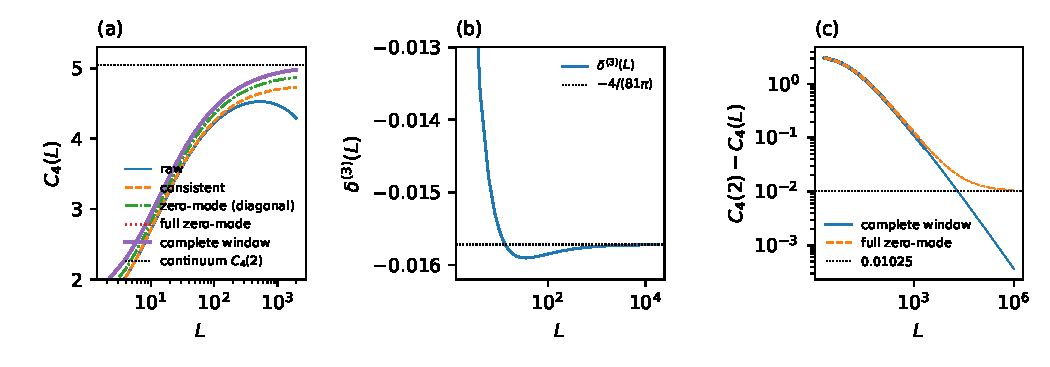
\includegraphics[width=\textwidth]{fig_c4_delta_d2.pdf}
\caption{(a) Exact $C_4(L)$ in $d=2$ for $L\le\HTpTwoLfour$ in five windows: raw, consistent, diagonal zero-mode, full
zero-mode (diagonal and off-diagonal) and complete; only the complete window converges to $C_4^{(2)}$ (dotted). (b) The
$\eps^3$ external-line coefficient $\delta^{(3)}(L)$ of Eq.~\eqref{d2:eq:delta} for $L\le\NTwoDeltaLmax$, with its limit
$-4/(81\pi)$ (dotted); it is not monotone. (c) Distance to the continuum value, $C_4^{(2)}-C_4(L)$, for the complete window
(solid) and the full zero-mode window (dashed); thin lines continue each with its tail fit $T_{22}$ ($300\le L\le2000$,
Appendix~\ref{d2:app:window}). The complete window falls like $\ln^2L/L$; the full zero-mode window levels off at
$0.01025$ (dotted), the part that the mass window $D^M$ supplies. Script \code{make\_fig\_d2.py}.}
\label{d2:fig}
\end{figure}

\subsection{Fifth order}\label{d2:c5}
\emph{All-order window and double counting.} At all orders $D^{\rm zm}$ uses the Bloch matrix of the auxiliary channels
$|z\rangle$ at sub-cutoff $\lambda$, $h(\lambda)=U\,{\rm diag}(E_z(\lambda))\,U^{-1}$ with $U_{z'z}=\langle z'|\psi_z(\lambda)\rangle$, and the mass
window is $D^M=\frac14\{e_1(L)-e_1(L-\hat\ell),M'\}$ with the Newton coefficient $e_1(\lambda)=E_1(\lambda)-E_0(\lambda)$; degenerate partners of $|z\rangle$
($z\ge5$) are projected out. If the auxiliary objects carry their own windows self-consistently, $C_5^W(L)$ diverges linearly,
with coefficient $\NTwoCfiveWLin\pm0.0004$ (the uncertainty of the linear term of raw $C_5$; Table~\ref{d2:tab:c5lin}). The cause is a double counting: a sunset nested in an auxiliary channel is restored once by
the outer $D^M$ and once more inside $h(L-\ell)$. Rule $W_c$ removes it: an auxiliary channel at sub-cutoff $\lambda<L$
represents a zero-mode cluster inside a state of the cutoff-$L$ theory, so its windows are referred to the outer cutoff,
$[h(L)-h(\lambda-\ell_\chi)]$ and $\frac14\{e_1(L)-e_1(\lambda-\hat\ell),M'\}$. It leaves $C_4$ unchanged and removes the linear term (Appendices~\ref{d2:app:Wall} to~\ref{d2:app:tests}).

\emph{External-line window.} In $W_c$ the $\eps^3$ spacing of $\chi_{aa}$ (Sec.~\ref{d2:desc}) tends to a constant,
$R_3\approx\NTwoRthreeWcConst\,a\,w_{aa}$ ($0.062$ to $0.063\,a\,w_{aa}$ at $L=16$ for $a=1$, 2, 3, changing slowly with $L$). An exact test with a tagged external line (Appendix~\ref{d2:app:tag}) locates it: if the external quantum is
invisible to the cutoff and the windows (budget-free), $R_3\to0$; if it is charged its level, $R_3$ reproduces its value
in $W_c$. $D^M$
charges both legs of a mass sub-process with their average level in every slice, which is exact for the $\eps^2$ sunset but not
for the mixed orderings at $\eps^3$. Scheme $W_{cs}$ adds at $\eps^3$
\begin{equation}
 D^{(3)}\mathrel{+}=\frac{\delta^{(3)}(L)}2\,X_0,\qquad \delta^{(3)}(L)=\tfrac14\big[e_1^{(3)}(L-2)-e_1^{{\rm tag},(3)}(L;2,2)\big] ,
 \label{d2:eq:wcs}
\end{equation}
where $X$ is $M'$ with each term multiplied by the summed level of its $\chi$ legs (plus for hops, minus for pair
creation and annihilation), $X_0$ its $\eps^0$ part, and $e_1^{\rm tag}(\lambda;2,2)$ is $E-E_0$ of the $\phi$ channel $|1\rangle$
at cutoff $\lambda$ whose external zero-mode quantum is tagged with charges $(2,2)$: it has level 0 in $H_0$, but the cutoff
and the windows count it as level 2 before it is absorbed and after it is re-emitted (Appendix~\ref{d2:app:wcs}). $\delta^{(3)}(L)$ is an exact rational at each $L$, one number per cutoff; nothing is
fitted (Appendix~\ref{d2:app:wcs} derives the operator form). Chain sums give it for every even $L\le\NTwoDeltaLmax$ (equal to the rationals at $L\le16$ to $\NTwoDeltaRational$).
It is not monotone, with a minimum $\NTwoDeltaMin$ at $L=\NTwoDeltaMinL$ (Fig.~\ref{d2:fig}b), and
\begin{equation}
 \delta^{(3)}(L)=-\frac4{81\pi}-\frac1{54\pi}\,\frac{\ln L}L+\mathcal O(1/L) ,
 \label{d2:eq:delta}
\end{equation}
where the limit $\delta_\infty=-\frac4{81\pi}$ (to $\NTwoDeltaIdent$ by free-limit fits) and the $\ln L/L$ coefficient are
identified numerically, not derived. With this identification the shift $4a\,w_{aa}\delta_\infty=-\frac{16}{81\pi}a\,w_{aa}$
of $R_3(\chi_{aa})$ that the window produces is two thirds of the $\eps^2$ exchange-sunset defect $\frac{8}{27\pi}a\,w_{aa}$
of $R_2$, and $\frac{16}{81\pi}=0.0629$ is close to the $W_c$ remainder above. The shift is therefore expected to cancel
that remainder as $L\to\infty$; this is not established, since $R_3$ is known only to $L=16$. $W_{cs}$ leaves $C_0$ to
$C_4$, $r_{\le3}$ and $g_{\le3}$ unchanged and shifts $C_5$ by $\delta^{(3)}(L)S(L)$, with $S(L)$ the $C_5$ response to
$\frac12X_0$; $S$ has no $\ln L$ and $S_\infty\equiv S(\infty)=\NTwoSinf$, so the shift tends to
$\delta_\infty S_\infty=\NTwoDeltaS$.

\emph{Data and tail} (Appendix~\ref{d2:app:c5tail}). $C_5^{W_{cs}}(L)$ is raw $C_5$ to $L=\HTpTwoLfive$ plus the exact $W_c$ shift and $\delta^{(3)}S$ (both
known to $L=\NTwoShiftLmax$). The tails of $C_2$ to $C_4$ carry $\ln^{n-2}L/L$, and hold-out tests select $\ln^3L/L$ for $C_5$. The
fits use
\begin{equation}
 C_5(L)=A+\sum_{j=0}^{3}a_j\frac{\ln^jL}{L}+\sum_{j=0}^{k_2}a'_j\frac{\ln^jL}{L^2},\qquad k_2\in\{0,1,2\},
 \label{d2:eq:C5tower}
\end{equation}
with no $\ln L$ term, on every even $L$ from $L_{\min}\in\{30,40,60,80,100\}$ to 300. Fitted to $L\le200$, these forms
predict $L=202$ to 300 to $\NTwoBlindNoLog$, against $\NTwoBlindFreeLog$ with a free $\ln L$; fitted to $L\le240$, both
predict $L=242$ to 300 to about $6\times10^{-7}$ (Appendix~\ref{d2:app:c5tail}). The median and half range
of the 15 fits give
\begin{equation}
 C_5=\HTpCfiveTwo\qquad\text{against}\qquad C_5^{(2)}=-38.8336459 ,
 \label{d2:eq:C5}
\end{equation}
with the unrounded median $\NTwoCfiveMedian$, $0.0018$ below the continuum value. Towers with one more power of $\ln L$
at $1/L$ ($k_1=4$), which the hold-out test does not exclude, move the median by only $\NTwoCfiveKfourShift$ but widen the half range
of the fits from $0.013$ to $\NTwoCfiveKfourHalf$ (Appendix~\ref{d2:app:c5tail}); the quoted uncertainty does not include
this. Without the external-line window,
$C_5^{W_c}=\NTwoCfiveWc$ (median $\NTwoCfiveWcMedian$), higher by about $-\delta_\infty S_\infty$ as expected. Both agree
with the continuum value within the spread of the fits, so $C_5$ does not distinguish $W_c$ from $W_{cs}$; the case for
the external-line window rests on the spacing $R_3$ (Sec.~\ref{d2:desc}).

\emph{Residual logarithm.}\label{d2:c5log} A term $b\ln L$ that the data cannot see would move the limit. Over the 15
fits of Eq.~\eqref{d2:eq:C5tower}, the median of the free coefficient drifts from $\NTwoBfreeTwoHundred$ at $L_{\max}=200$
to $\NTwoBfreeThreeHundred$ at 300; a second set of twelve fits ($L_{\min}=30$ to 80) drifts from $-0.0134$ to $+0.0054$
(Appendix~\ref{d2:app:c5tail}). On $C_4^W$, which has no $\ln L$, the 15-fit estimator returns $\NTwoBnull$. On a synthetic
series with a $C_5$-like tail and a known $b$, both sets read about $\NTwoBbias$ low; corrected for this bias, the median
is about $\NTwoBcorr$ (15 fits; $+0.009$ with 12). We take $|b|\lesssim\NTwoBbound$ as a judgement from this median, its
drift and its bias; it is not a confidence bound. The individual fits of the 15-fit set range from $\NTwoBfitMin$ to
$\NTwoBfitMax$, but the extreme ones have nearly as many parameters as points; taken as a bound they would allow shifts of
$C_5$ between about $-0.7$ and $+0.5$. In the 15 fits, fixing $b=\mp\NTwoBbound$ moves the limit by about
$\pm\HTpCfiveTwoLog$, and $b=\NTwoBcorr$ would move it by about $-0.08$; bounding $|b|$ well below $\NTwoBbound$ would
need $L\gtrsim\NTwoLneeded$. The external-line class itself gives no $\ln L$: the
$\ln L$ terms of $S$ cancel within the hop and within the pair sector separately.

\emph{Status.} The complete window has no fitted parameter, removes the $\ln L$ and is verified through $\eps^4$. At $\eps^5$
the rule $W_c$ is needed to remove a linear divergence, and the external-line window to reduce $R_3$ (by at least
$\HTpTwoIdentThree\%$ at $L=14$ and 16). With both, $C_5$ agrees with the continuum. Both rules are provisional: they are
not derived in full, and the window is not proven complete at this order. Like all windows here, they were derived after
their effect had been seen and with the continuum values known.

\subsection{Descendant spacings}\label{d2:desc}
A descendant lies an integer above its primary at every order. With
\begin{equation}
 R_n(L)=\big[E(\chi_{aa})-E(\phi)-2a\big]_{\eps^n},
 \label{d2:eq:R}
\end{equation}
the $\eps^n$ coefficient of the spacing of $\chi_{aa}=\partial^a\bar\partial^a\phi$ computed with the same $r$, $g$ and
window, and the same for the descendants $(\partial\bar\partial)^a\phi^2$ of $\phi^2$, the exact small-$L$ solvers
\code{complete\_exact} and \code{ce\_wc} (Sec.~\ref{d2:solvers}) give every $R_n$, $n\le8$, as rationals for $L\le16$ in each
scheme. These tests need no continuum input; Appendix~\ref{d2:app:legs} gives the data.
\begin{itemize}
\item $\eps^2$: in the consistent and zero-mode windows the exchange sunset of $\chi_{aa}$ has only $L-4a$, and
 $R_2\to\frac{8a\,w_{aa}}{27\pi}$ ($\NTwoRtwoCons$ for $\chi_{11}$ at $L=16$). $D^M$ shifts it by exactly
 $-\frac{8a\,w_{aa}}{27\pi}$, so in the complete window $R_2$ decays like $1/L$ ($\NTwoRtwoWcoef/L$ for $\chi_{11}$), also for
 the $\phi^2$ descendants.
\item $\eps^3$, single-quantum descendants: $R_3(\chi_{11})$ is $\NTwoRthreeWcSixteen$ in $W_c$ and $\NTwoRthreeWcsSixteen$ in
 $W_{cs}$ at $L=16$. At $L=14$ and 16 the window leaves at most 3\% of the $W_c$ value for $a=1$ to 3, so at least
 $\HTpTwoIdentThree\%$ of the defect is removed at $L=14$ and 16. Free-limit fits of $\chi_{11}$ leave a few percent, and the window is
 expected to cancel the defect as $L\to\infty$ (above); $R_3$ itself is not computed beyond
 $L=16$.
\item $\eps^3$, descendants of $\phi^2$: at $L=16$, $R_3=\NTwoPhiDescTwo$ (level 2) and $\NTwoPhiDescFour$ (level 4) in $W_{cs}$;
 the level-4 value still moves away from zero. Not settled.
\item $\eps^4$: in $W_c$ and $W_{cs}$, $R_4(\chi_{11})$ grows, with a local slope of about $\NTwoRfourSlope$ per unit of $\ln L$
 at $L=8$ to 16, while with budget-free legs it goes
 to zero: the same leg defect one order higher. A partial $\chi$-line window ($W_{cs4\chi}$, calibrated on $\chi_{11}$, with the
 $\eps^4$ difference between the $\chi$-line and zero-mode self-energies as a spectator term) closes $\NTwoGapTwo\%$ and
 $\NTwoGapThree\%$ of the gaps of $\chi_{22}$ and $\chi_{33}$ to their budget-free lines at $L=14$, but the $\chi_{22}$ gap is not
 shrinking, the $\phi^2$ descendants still grow, and $R_5(\chi_{aa})$ grows. The window coefficient grows roughly like $\ln L$
 at $L\le16$, which suggests that
 $C_6$ in $W_c$ carries about $\NTwoCsixLog\ln L$ (a prediction, not a measurement). The $\eps^4$ window is not yet known.
\end{itemize}

\subsection{Sixth to eighth order}\label{d2:c6}
$C_6$ to $C_8$ are not reproduced. At $L=16$, $C_6\approx\NTwoCsixSixteen$ in $W_c$, $W_{cs}$ and $W_{cs4\chi}$
(Table~\ref{d2:tab:c6}), $54\%$ below the continuum value $\NTwoCsixCont$, and $C_6(L)$ still rises by about
$\NTwoCsixStep$ per step of 2 in $L$. The external-line windows shift $C_6$ by about $10^{-4}$ of its value there, while
$W$ and $W_c$ differ by about 1\% (Appendix~\ref{d2:app:c6eps5}). The production tables to $L=\HTpTwoLprod$ (raw and
consistent) are shipped as finite-cutoff data, but those windows diverge from $\eps^4$ on, and the external-line windows
from $\eps^4$ on are not known.
